% !Mode:: "TeX:UTF-8"
% 请注意,此文件的编码方式一定要设置为UTF-8 无DOM模式
% 否则中文显示乱码!
% 可以用notepad++ 或ultraedit查看/更改文件编码方式

\documentclass[a4paper,12pt]{article}

%插入超链接,并且去除超链接的颜色下划线等特性
\usepackage[hidelinks]{hyperref}

%该宏包可以添加伪代码CLRS《算法导论》**第三版**模式
%clrscode3e.sty放在项目根目录下即可
\usepackage{clrscode3e}

%插入数学公式
\usepackage{amsmath}

%中文包
\usepackage{xeCJK}
\setCJKmainfont{SimSun}

%设置页边距
\usepackage[top=0.93in,bottom=0.8in,left=1.1in,right=1in]{geometry}

\usepackage{xcolor}

%为了插入代码
\usepackage{listings}

\definecolor{codegreen}{rgb}{0,0.6,0}
\definecolor{codegray}{rgb}{0.5,0.5,0.5}
\definecolor{codepurple}{rgb}{0.58,0,0.82}
\definecolor{backcolour}{rgb}{0.95,0.95,0.92}

\lstdefinestyle{mystyle}{
    backgroundcolor=\color{backcolour},
    commentstyle=\itshape\color{codegreen},
    keywordstyle=\color{magenta},
    numberstyle=\tiny\color{codegray},
    stringstyle=\color{codepurple},
    basicstyle=\footnotesize,
    breakatwhitespace=false,
    breaklines=true,
    captionpos=b,
    keepspaces=true,
    numbers=left,
    numbersep=5pt,
    showspaces=false,
    showstringspaces=false,
    showtabs=false,
    tabsize=4
}

\lstdefinestyle{default}{
    backgroundcolor=\color{backcolour},
    commentstyle=\itshape,
    numberstyle=\tiny,
    basicstyle=\footnotesize,
    breakatwhitespace=false,
    breaklines=true,
    captionpos=b,
    keepspaces=true,
    numbers=left,
    numbersep=5pt,
    showspaces=false,
    showstringspaces=false,
    showtabs=false,
    tabsize=4
}

\lstset{style=default}

%为了插入图片
%\usepackage{graphicx}

%为了画图
\usepackage{tikz}
\usetikzlibrary{positioning}

%插入表格,自定义表格横竖线
\usepackage{tabularx,hhline}% http://ctan.org/pkg/{tabularx,hhline}

%数学符号,三角形△
\usepackage{amssymb}

%首段缩进
\usepackage{indentfirst}

\title{Assignment 6\\Algorithm Design and Analysis}

\author{\href{http://bitjoy.net}{bitjoy.net}}
\date{January 2, 2016}

\begin{document}

\maketitle

I choose problem 1,2,3,4,5,6.

\section*{1\quad Integer Programming}

We first show that Integer Programming is in \textbf{NP}. Obviously, given an $n$-vector $x$, $Ax\geq b$ can be verified in polynomial time, so it is in \textbf{NP}.

We then prove that $3SAT\leq_p ILP$. Given a $3SAT$ instance like this:

\[
(x_1\vee x_2 \vee x_3)\land(x_1\vee \lnot x_2\vee x_4)\tag{1}
\]

We will have corresponding variables $y_1,y_2,y_3,y_4$ in our \emph{ILP}, if $x_i=true$, then $y_i=1$ otherwise $y_i=0$.

\[
\begin{array}{rrrcl}
 \max & 0&   \\
 s.t. & y_1+y_2+y_3 &\geq & 1 &  \\ \tag{2}
      & y_1+(1-y_2)+y_4 &\geq & 1 & \\
      & y_i &\in & \{0,1\}& i=1,...,4
\end{array} \nonumber
\]

If (1) can be satisfied, the corresponding $y_i$s are the optimal solution to (2), that's to say (2) has optimal solution. If (2) has optimal solution, the corresponding $x_i$s make (1) be $true$. If (1) can't be satisfied, (2) has no optimal solution, and vice versa. So, $3SAT\leq_p ILP$.

Integer-programming is in \textbf{NP}-complete.

\section*{2\quad Mine-sweeper}
Here is the MINESWEEPER language:

MINESWEEPER: \{$G,\xi$ | $G$ is a graph and $\xi$ is a partial integer labeling of $G$, and $G$ can be filled with mines in such a way that any node $v$ labeled $m$ has exactly $m$ neighboring nodes containing mines.\}

Deciding if a graph is in the MINESWEEPER language is \textbf{NP}-complete.

First, given a graph with nodes labeled with integers or containing mines, we can verify it in polynomial time. Just check whether each node labeled with $m$ has exactly $m$ neighboring nodes containing mines.

Second, we prove $3SAT\leq_p MINESWEEPER$. Suppose we have one $3SAT$ clause
\[
(x_1\vee\lnot x_2\vee x_3)\tag{3}
\]
For each variable, we construct a gadget like Figure 1.

%http://tex.stackexchange.com/questions/8652/what-does-t-and-ht-mean
\begin{figure}[!ht]
\centering
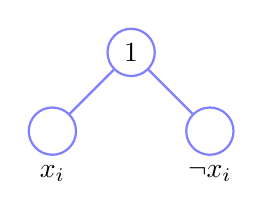
\begin{tikzpicture}
    [mine/.style={circle, draw=red!50,fill=red!70,thick,inner sep=0pt,minimum size=6mm},
    empty/.style={circle, draw=blue!50,thick,inner sep=0pt,minimum size=6mm}]
    \node[empty] (root) at (0,0) {1};
    \node[empty,label=below:{$x_i$}] (left) at (-1,-1) {};
    \node[empty,label=below:{$\lnot x_i$}] (right) at (1,-1) {};

    \draw [blue!50,thick] (root) -- (left);
    \draw [blue!50,thick] (root) -- (right);
\end{tikzpicture}
\caption{Gadget for each variable.}
\end{figure}

If $x_i=true$, then $x_i$ is filled with mine, otherwise $\lnot x_i$ is filled with mine. The top node labeled with '1' forces that only one of $x_i$ and $\lnot x_i$ can be $true$.

For clause (3), we have:
%http://tex.stackexchange.com/questions/8652/what-does-t-and-ht-mean
\begin{figure}[!ht]
\centering
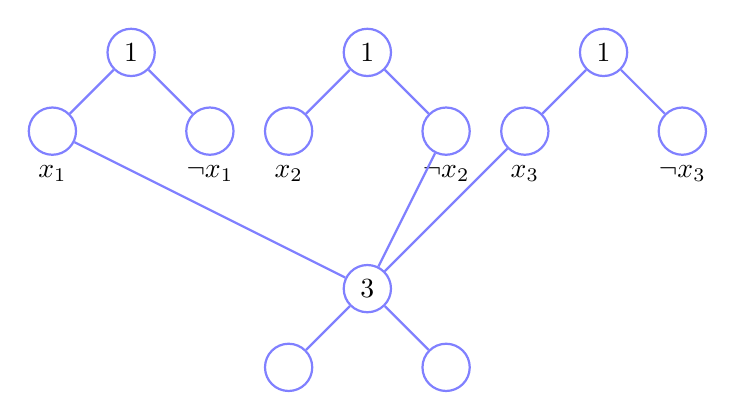
\begin{tikzpicture}
    [mine/.style={circle, draw=red!50,fill=red!70,thick,inner sep=0pt,minimum size=6mm},
    empty/.style={circle, draw=blue!50,thick,inner sep=0pt,minimum size=6mm}]
    \node[empty] (rx2) at (0,0) {1};
    \node[empty,label=below:{$x_2$}] (x2) at (-1,-1) {};
    \node[empty,label=below:{$\lnot x_2$}] (notx2) at (1,-1) {};
    \node[empty] (rx3) at (3,0) {1};
    \node[empty,label=below:{$x_3$}] (x3) at (2,-1) {};
    \node[empty,label=below:{$\lnot x_3$}] (notx3) at (4,-1) {};
    \node[empty] (rx1) at (-3,0) {1};
    \node[empty,label=below:{$x_1$}] (x1) at (-4,-1) {};
    \node[empty,label=below:{$\lnot x_1$}] (notx1) at (-2,-1) {};
    \node[empty] (root) at (0,-3) {3};
    \node[empty] (left) at (-1,-4) {};
    \node[empty] (right) at (1,-4) {};

    \draw [blue!50,thick] (rx2) -- (x2);
    \draw [blue!50,thick] (rx2) -- (notx2);
    \draw [blue!50,thick] (rx1) -- (x1);
    \draw [blue!50,thick] (rx1) -- (notx1);
    \draw [blue!50,thick] (rx3) -- (x3);
    \draw [blue!50,thick] (rx3) -- (notx3);
    \draw [blue!50,thick] (root) -- (left);
    \draw [blue!50,thick] (root) -- (right);
    \draw [blue!50,thick] (root) -- (x1);
    \draw [blue!50,thick] (root) -- (notx2);
    \draw [blue!50,thick] (root) -- (x3);
\end{tikzpicture}
\caption{Gadget for each clause.}
\end{figure}

For each $true$ assignment of this clause, we can find a placement of mines makes the graph consistent. Figure 3 is one of $true$ assignment examples.
%http://tex.stackexchange.com/questions/8652/what-does-t-and-ht-mean
\begin{figure}[!ht]
\centering
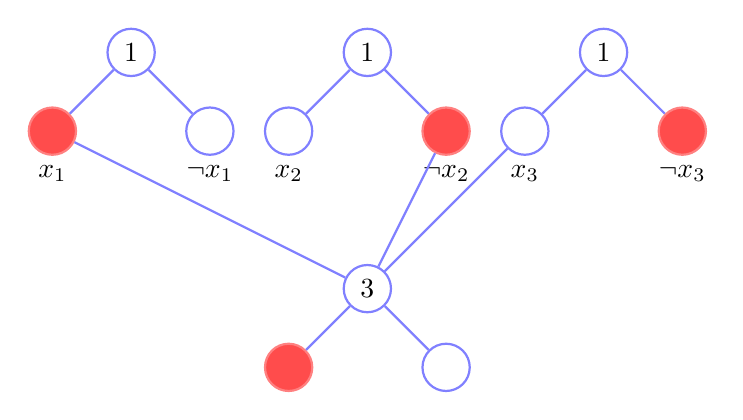
\begin{tikzpicture}
    [mine/.style={circle, draw=red!50,fill=red!70,thick,inner sep=0pt,minimum size=6mm},
    empty/.style={circle, draw=blue!50,thick,inner sep=0pt,minimum size=6mm}]
    \node[empty] (rx2) at (0,0) {1};
    \node[empty,label=below:{$x_2$}] (x2) at (-1,-1) {};
    \node[mine,label=below:{$\lnot x_2$}] (notx2) at (1,-1) {};
    \node[empty] (rx3) at (3,0) {1};
    \node[empty,label=below:{$x_3$}] (x3) at (2,-1) {};
    \node[mine,label=below:{$\lnot x_3$}] (notx3) at (4,-1) {};
    \node[empty] (rx1) at (-3,0) {1};
    \node[mine,label=below:{$x_1$}] (x1) at (-4,-1) {};
    \node[empty,label=below:{$\lnot x_1$}] (notx1) at (-2,-1) {};
    \node[empty] (root) at (0,-3) {3};
    \node[mine] (left) at (-1,-4) {};
    \node[empty] (right) at (1,-4) {};

    \draw [blue!50,thick] (rx2) -- (x2);
    \draw [blue!50,thick] (rx2) -- (notx2);
    \draw [blue!50,thick] (rx1) -- (x1);
    \draw [blue!50,thick] (rx1) -- (notx1);
    \draw [blue!50,thick] (rx3) -- (x3);
    \draw [blue!50,thick] (rx3) -- (notx3);
    \draw [blue!50,thick] (root) -- (left);
    \draw [blue!50,thick] (root) -- (right);
    \draw [blue!50,thick] (root) -- (x1);
    \draw [blue!50,thick] (root) -- (notx2);
    \draw [blue!50,thick] (root) -- (x3);
\end{tikzpicture}
\caption{$\{x_1=true,x_2=false,x_3=false\}$ is one of true assignment for clause (3), we find a placement of mines makes the graph consistent.}
\end{figure}

For the $false$ assignment of this clause, we can't find any placement of mines makes the graph consistent. Figure 4 is the $false$ assignment.
%http://tex.stackexchange.com/questions/8652/what-does-t-and-ht-mean
\begin{figure}[!ht]
\centering
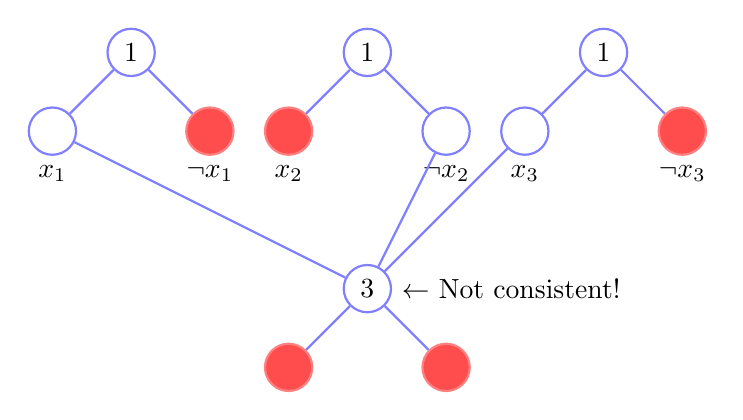
\begin{tikzpicture}
    [mine/.style={circle, draw=red!50,fill=red!70,thick,inner sep=0pt,minimum size=6mm},
    empty/.style={circle, draw=blue!50,thick,inner sep=0pt,minimum size=6mm}]
    \node[empty] (rx2) at (0,0) {1};
    \node[mine,label=below:{$x_2$}] (x2) at (-1,-1) {};
    \node[empty,label=below:{$\lnot x_2$}] (notx2) at (1,-1) {};
    \node[empty] (rx3) at (3,0) {1};
    \node[empty,label=below:{$x_3$}] (x3) at (2,-1) {};
    \node[mine,label=below:{$\lnot x_3$}] (notx3) at (4,-1) {};
    \node[empty] (rx1) at (-3,0) {1};
    \node[empty,label=below:{$x_1$}] (x1) at (-4,-1) {};
    \node[mine,label=below:{$\lnot x_1$}] (notx1) at (-2,-1) {};
    \node[empty,label=right:{$\leftarrow$ Not consistent!}] (root) at (0,-3) {3};
    \node[mine] (left) at (-1,-4) {};
    \node[mine] (right) at (1,-4) {};

    \draw [blue!50,thick] (rx2) -- (x2);
    \draw [blue!50,thick] (rx2) -- (notx2);
    \draw [blue!50,thick] (rx1) -- (x1);
    \draw [blue!50,thick] (rx1) -- (notx1);
    \draw [blue!50,thick] (rx3) -- (x3);
    \draw [blue!50,thick] (rx3) -- (notx3);
    \draw [blue!50,thick] (root) -- (left);
    \draw [blue!50,thick] (root) -- (right);
    \draw [blue!50,thick] (root) -- (x1);
    \draw [blue!50,thick] (root) -- (notx2);
    \draw [blue!50,thick] (root) -- (x3);
\end{tikzpicture}
\caption{$\{x_1=false,x_2=true,x_3=false\}$ is the false assignment for clause (3), we can't find any placement of mines makes the graph consistent.}
\end{figure}

\newpage
So, if $3SAT$ can be satisfied, graph $G$ is in the MINESWEEPER language, otherwise not.

Mine-sweeper is in \textbf{NP}-complete.

\section*{3\quad Half-3SAT}

First, Half-3SAT is in \textbf{NP}. Given a particular assignment of $n$ variables, we can check if $m$ clauses satisfy Half-3SAT conditions in polynomial time. Just check each clause, if half are $true$, half are $false$, it's Half-3SAT, otherwise not.

Second, we prove $3SAT\leq_p Half-3SAT$. Given a instance of $3SAT$ with $m$ clauses, we construct a $Half-3SAT$ instance with $4m$ clauses like this. First $m$ clauses are exactly the same as $3SAT$. Next, we create $m$ clauses of the form
\[
(p\vee\lnot p\vee q)\tag{4}
\]
which is always $true$. Next, we create $2m$ of clauses of the form
\[
(p\vee q\vee r)\tag{5}
\]
These $2m$ clauses are always $true$ or always $false$.

If $3SAT$ is satisfied, we set last $2m$ clauses be $false$. So there are $2m~true$ clauses and $2m~false$ clauses. Thus, $Half-3SAT$ is satisfied.

If $Half-3SAT$ is satisfied, as there are $m$ (4) clauses, which is always $true$, so the last $2m$ (5) clauses can only be $false$. Thus, the first $m$ clauses are $true$, $3SAT$ is satisfied.

Half-3SAT is in \textbf{NP}-complete.

\section*{4\quad Solitaire Game}

First, Solitaire Game is in \textbf{NP}. Given a final board status, we can determine whether it satisfies the winning condition in polynomial time. Just check whether each column contains only stones of a single color and each row contains at least one stone. For $n\times n$ board, it takes $O(2n)$, so Solitaire Game is in \textbf{NP}.

Second, we prove $3SAT\leq_p SOLITAIRE$. Given a instance of $3SAT$ with
2 clauses and 4 variables:
\[
(x_1\vee x_2 \vee x_3)\land (x_1\vee \lnot x_2\vee x_4)\tag{6}
\]

\newcommand{\bstone}{$\begingroup\color{blue}{\blacktriangle}\endgroup$}
\newcommand{\rstone}{$\begingroup\color{red}{\blacksquare}\endgroup$}

For each variables, \bstone for $x_i$ and \rstone for $\lnot x_i$. So we get Table 1 for (6).

%http://tex.stackexchange.com/questions/180064/remove-vertical-lines-in-the-table-unsuccessfully
\begin{table}[!ht]
\centering
\begin{tabular}{c|c|c|c|c|}
\multicolumn{1}{c}{}& \multicolumn{1}{c}{$x_1$} & \multicolumn{1}{c}{$x_2$} & \multicolumn{1}{c}{$x_3$} & \multicolumn{1}{c}{$x_4$}\\
\hhline{~----}
$c_1$ & \bstone & \bstone & \bstone &   \\
\hhline{~----}
$c_2$ & \bstone & \rstone &  & \bstone  \\
\hhline{~----}
$\times$ & $\times$ & $\times$ & $\times$ & $\times$  \\
\hhline{~----}
$\times$ & $\times$ & $\times$ & $\times$ & $\times$  \\
\hhline{~----}
\end{tabular}
\caption{Initial board for (6), \bstone for $x_i$ and \rstone for $\lnot x_i$, one row for one clause.}
\end{table}

For $(y_1\vee y_2\vee y_3)$, $y_i$ can be $x_j$ or $\lnot x_j$. For each clause, if $y_i=false$, we remove the corresponding stone. If (6) can be satisfied, then Table 1 is a winnable game configuration. Table 2 is one of $true$ examples.
%http://tex.stackexchange.com/questions/180064/remove-vertical-lines-in-the-table-unsuccessfully
\begin{table}[!ht]
\centering
\begin{tabular}{c|c|c|c|c|}
\multicolumn{1}{c}{}& \multicolumn{1}{c}{$x_1$} & \multicolumn{1}{c}{$x_2$} & \multicolumn{1}{c}{$x_3$} & \multicolumn{1}{c}{$x_4$}\\
\hhline{~----}
$c_1$ & \bstone & \bstone & \bstone &   \\
\hhline{~----}
$c_2$ & \bstone &  &  & \bstone  \\
\hhline{~----}
$\times$ & $\times$ & $\times$ & $\times$ & $\times$  \\
\hhline{~----}
$\times$ & $\times$ & $\times$ & $\times$ & $\times$  \\
\hhline{~----}
\end{tabular}
\caption{$\{x_1=true,x_2=true,x_3=true,x_4=true\}$ is the true assignment for clause (6), $\lnot x_2=false$, so removing the red stone in $c_2$, we win the game.}
\end{table}

For any $false$ assignment of (6), Table 1 is not a winnable game configuration. Table 3 is one of $false$ examples.

%http://tex.stackexchange.com/questions/180064/remove-vertical-lines-in-the-table-unsuccessfully
\begin{table}[!ht]
\centering
\begin{tabular}{c|c|c|c|c|}
\multicolumn{1}{c}{}& \multicolumn{1}{c}{$x_1$} & \multicolumn{1}{c}{$x_2$} & \multicolumn{1}{c}{$x_3$} & \multicolumn{1}{c}{$x_4$}\\
\hhline{~----}
$c_1$ &  & \bstone & \bstone &   \\
\hhline{~----}
$c_2$ &  &  &  &   \\
\hhline{~----}
$\times$ & $\times$ & $\times$ & $\times$ & $\times$  \\
\hhline{~----}
$\times$ & $\times$ & $\times$ & $\times$ & $\times$  \\
\hhline{~----}
\end{tabular}
\caption{$\{x_1=false,x_2=true,x_3=true,x_4=false\}$ is the false assignment for clause (6), similarily, removing $<c_1,x_1>,<c_2,x_1>,<c_2,x_2>,<c_2,x_4>$, we lose the game.}
\end{table}

So, if $3SAT$ can be satisfied, $G$ is a winnable game configuration, otherwise not.

Solitaire Game is in \textbf{NP}-complete.

\section*{5\quad Directed Disjoint Paths Problem}
First, Directed Disjoint Paths Problem is in \textbf{NP}. Given $k$ paths $P_1,P_2,...,P_k$, we can determine whether they are Directed Disjoint Paths in polynomial time. Just go through every path and record the nodes, if more than one path go through a node, they are not Disjoint Paths.

Second, we prove $3SAT\leq_p Directed~Disjoint~Paths~Problem$. Given an arbitrary $3SAT$ formula, we construct a network routing problem like this: For each clause $C_i$, we create a source/sink pair $(s_i,t_i)$, and a node $x^i_j$($\lnot x^i_j$) for each literal $x_j$($\lnot x_j$) in the clause. Add edges $<s_i,x^i_j>$ and edges $<x^i_j,t_i>$. In addition, we create source/sink pair $(s_j,t_j)$ for each variable $x_j$, we get a total of $k=q+n$ source/sink pairs, where $q$ is the number of clauses and $n$ is the number of literals.

For example, given a $3SAT$ instance with two clauses and three variables:
\[
(x_1\vee \lnot x_2 \vee x_3)\land (\lnot x_1\vee x_2\vee x_3)\tag{7}
\]
We construct a graph $G$ like Figure 5.
%http://tex.stackexchange.com/questions/8652/what-does-t-and-ht-mean
\begin{figure}[!ht]
\centering
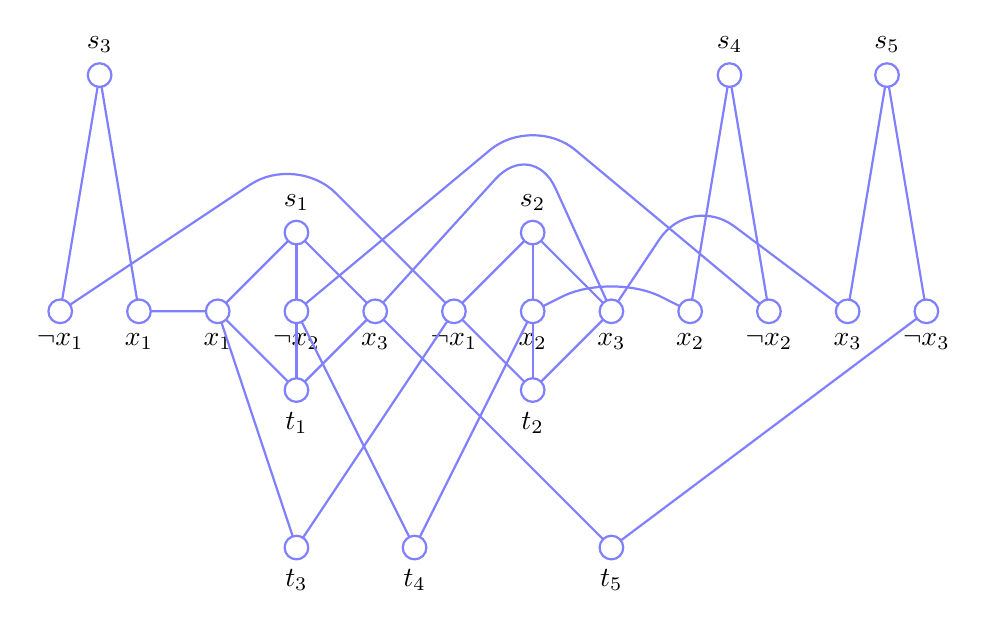
\begin{tikzpicture}
    [mine/.style={circle, draw=red!50,fill=red!70,thick,inner sep=0pt,minimum size=6mm,scale=0.5},
    empty/.style={circle, draw=blue!50,thick,inner sep=0pt,minimum size=6mm,scale=0.5}]
    \node[empty,label=below:{$x_1$}] (x11) at (0,0) {};
    \node[empty,label=below:{$\lnot x_2$}] (x12) at (1,0) {};
    \node[empty,label=below:{$x_3$}] (x13) at (2,0) {};
    \node[empty,label=above:{$s_1$}] (s1) at (1,1) {};
    \node[empty,label=below:{$t_1$}] (t1) at (1,-1) {};

    \node[empty,label=below:{$\lnot x_1$}] (x21) at (3,0) {};
    \node[empty,label=below:{$x_2$}] (x22) at (4,0) {};
    \node[empty,label=below:{$x_3$}] (x23) at (5,0) {};
    \node[empty,label=above:{$s_2$}] (s2) at (4,1) {};
    \node[empty,label=below:{$t_2$}] (t2) at (4,-1) {};

    \node[empty,label=below:{$x_1$}] (x31) at (-1,0) {};
    \node[empty,label=below:{$\lnot x_1$}] (nx31) at (-2,0) {};
    \node[empty,label=above:{$s_3$}] (s3) at (-1.5,3) {};
    \node[empty,label=below:{$t_3$}] (t3) at (1,-3) {};

    \node[empty,label=below:{$x_2$}] (x42) at (6,0) {};
    \node[empty,label=below:{$\lnot x_2$}] (nx42) at (7,0) {};
    \node[empty,label=above:{$s_4$}] (s4) at (6.5,3) {};
    \node[empty,label=below:{$t_4$}] (t4) at (2.5,-3) {};

    \node[empty,label=below:{$x_3$}] (x53) at (8,0) {};
    \node[empty,label=below:{$\lnot x_3$}] (nx53) at (9,0) {};
    \node[empty,label=above:{$s_5$}] (s5) at (8.5,3) {};
    \node[empty,label=below:{$t_5$}] (t5) at (5,-3) {};

    \draw [blue!50,thick] (s1) -- (x11);
    \draw [blue!50,thick] (s1) -- (x12);
    \draw [blue!50,thick] (s1) -- (x13);
    \draw [blue!50,thick] (t1) -- (x11);
    \draw [blue!50,thick] (t1) -- (x12);
    \draw [blue!50,thick] (t1) -- (x13);

    \draw [blue!50,thick] (s2) -- (x21);
    \draw [blue!50,thick] (s2) -- (x22);
    \draw [blue!50,thick] (s2) -- (x23);
    \draw [blue!50,thick] (t2) -- (x21);
    \draw [blue!50,thick] (t2) -- (x22);
    \draw [blue!50,thick] (t2) -- (x23);

    \draw [blue!50,thick] (s3) -- (x31);
    \draw [blue!50,thick] (s3) -- (nx31);

    \draw [blue!50,thick] (s4) -- (x42);
    \draw [blue!50,thick] (s4) -- (nx42);

    \draw [blue!50,thick] (s5) -- (x53);
    \draw [blue!50,thick] (s5) -- (nx53);
    \draw [blue!50,thick] (t5) -- (nx53);

    \draw [blue!50,thick,rounded corners=20pt] (x31) -- (x11) -- (t3);
    \draw [blue!50,thick,rounded corners=20pt] (nx31) -- (1,2)-- (x21) -- (t3);

    \draw [blue!50,thick,rounded corners=20pt] (x42) -- (5,0.5) -- (x22) -- (t4);
    \draw [blue!50,thick,rounded corners=20pt] (nx42) -- (4,2.5) -- (x12) -- (t4);

    \draw [blue!50,thick,rounded corners=20pt] (x53) -- (6,1.5) -- (x23) -- (4,2.2) -- (x13) -- (t5);

\end{tikzpicture}
\caption{Graph $G$ for $3SAT$ formula (7).}
\end{figure}

We now show that if $3SAT$ can be satisfied, there are node-disjoint paths for $k$ pairs of nodes $(s_i,t_i)$.

Given a $true$ assignment of $3SAT$, we construct the $k$ paths as follows. For each $(s_j,t_j)$ pair that representing a variable $x_j$, we choose the path that corresponds to the literal that is not set to true in the satisfying assignment. For example, if $x_j=true$, we choose path $(s_j,t_j)$ that goes through $\lnot x_j$, if $x_j=false$, we choose path $(s_j,t_j)$ that goes through $x_j$.

$\{x_1=true,x_2=true,x_3=false\}$ is a $true$ assignment of formula (7), according to rules above, we get Figure 6, which has $k=5$ node-disjoint paths.
%http://tex.stackexchange.com/questions/8652/what-does-t-and-ht-mean
\begin{figure}[!ht]
\centering
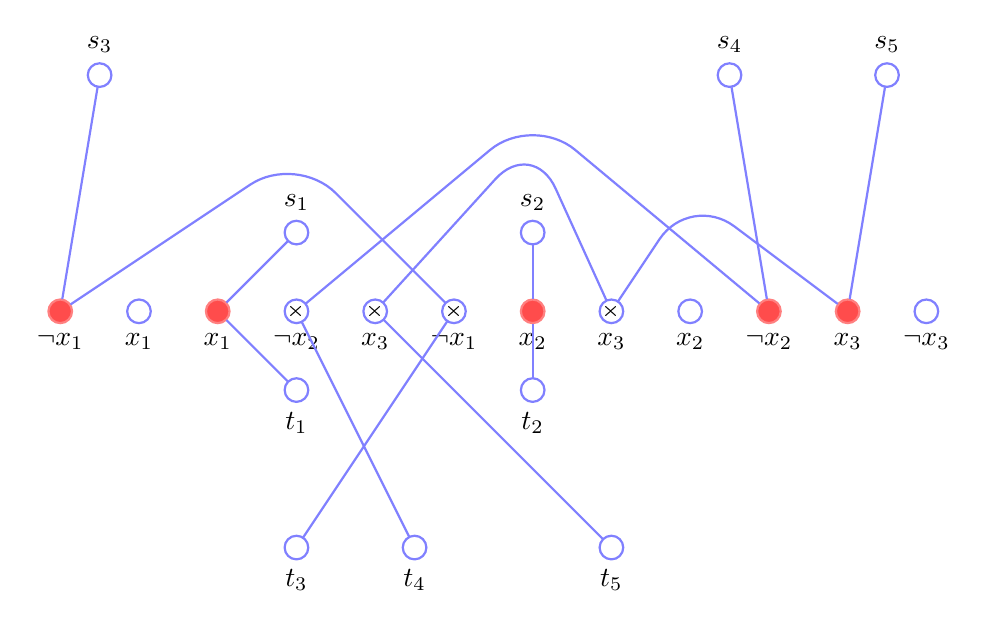
\begin{tikzpicture}
    [mine/.style={circle, draw=red!50,fill=red!70,thick,inner sep=0pt,minimum size=6mm,scale=0.5},
    empty/.style={circle, draw=blue!50,thick,inner sep=0pt,minimum size=6mm,scale=0.5}]
    \node[mine,label=below:{$x_1$}] (x11) at (0,0) {};
    \node[empty,label=below:{$\lnot x_2$}] (x12) at (1,0) {\Large\textbf{{×}}};
    \node[empty,label=below:{$x_3$}] (x13) at (2,0) {\Large\textbf{{×}}};
    \node[empty,label=above:{$s_1$}] (s1) at (1,1) {};
    \node[empty,label=below:{$t_1$}] (t1) at (1,-1) {};

    \node[empty,label=below:{$\lnot x_1$}] (x21) at (3,0) {\Large\textbf{{×}}};
    \node[mine,label=below:{$x_2$}] (x22) at (4,0) {};
    \node[empty,label=below:{$x_3$}] (x23) at (5,0) {\Large\textbf{{×}}};
    \node[empty,label=above:{$s_2$}] (s2) at (4,1) {};
    \node[empty,label=below:{$t_2$}] (t2) at (4,-1) {};

    \node[empty,label=below:{$x_1$}] (x31) at (-1,0) {};
    \node[mine,label=below:{$\lnot x_1$}] (nx31) at (-2,0) {};
    \node[empty,label=above:{$s_3$}] (s3) at (-1.5,3) {};
    \node[empty,label=below:{$t_3$}] (t3) at (1,-3) {};

    \node[empty,label=below:{$x_2$}] (x42) at (6,0) {};
    \node[mine,label=below:{$\lnot x_2$}] (nx42) at (7,0) {};
    \node[empty,label=above:{$s_4$}] (s4) at (6.5,3) {};
    \node[empty,label=below:{$t_4$}] (t4) at (2.5,-3) {};

    \node[mine,label=below:{$x_3$}] (x53) at (8,0) {};
    \node[empty,label=below:{$\lnot x_3$}] (nx53) at (9,0) {};
    \node[empty,label=above:{$s_5$}] (s5) at (8.5,3) {};
    \node[empty,label=below:{$t_5$}] (t5) at (5,-3) {};

    \draw [blue!50,thick] (s1) -- (x11);
    %\draw [blue!50,thick] (s1) -- (x12);
    %\draw [blue!50,thick] (s1) -- (x13);
    \draw [blue!50,thick] (t1) -- (x11);
    %\draw [blue!50,thick] (t1) -- (x12);
    %\draw [blue!50,thick] (t1) -- (x13);

    %\draw [blue!50,thick] (s2) -- (x21);
    \draw [blue!50,thick] (s2) -- (x22);
    %\draw [blue!50,thick] (s2) -- (x23);
    %\draw [blue!50,thick] (t2) -- (x21);
    \draw [blue!50,thick] (t2) -- (x22);
    %\draw [blue!50,thick] (t2) -- (x23);

    %\draw [blue!50,thick] (s3) -- (x31);
    \draw [blue!50,thick] (s3) -- (nx31);

    %\draw [blue!50,thick] (s4) -- (x42);
    \draw [blue!50,thick] (s4) -- (nx42);

    \draw [blue!50,thick] (s5) -- (x53);
    %\draw [blue!50,thick] (s5) -- (nx53);
    %\draw [blue!50,thick] (t5) -- (nx53);

    %\draw [blue!50,thick,rounded corners=20pt] (x31) -- (x11) -- (t3);
    \draw [blue!50,thick,rounded corners=20pt] (nx31) -- (1,2)-- (x21) -- (t3);

    %\draw [blue!50,thick,rounded corners=20pt] (x42) -- (5,0.5) -- (x22) -- (t4);
    \draw [blue!50,thick,rounded corners=20pt] (nx42) -- (4,2.5) -- (x12) -- (t4);

    \draw [blue!50,thick,rounded corners=20pt] (x53) -- (6,1.5) -- (x23) -- (4,2.2) -- (x13) -- (t5);

\end{tikzpicture}
\caption{When $\{x_1=true,x_2=true,x_3=false\}$, we find $k=5$ node-disjoint paths.}
\end{figure}

$\{x_1=false,x_2=true,x_3=false\}$ is a $false$ assignment of formula (7), according to rules above, we can't find $k=5$ node-disjoint paths. Figure 7 shows this case.
%http://tex.stackexchange.com/questions/8652/what-does-t-and-ht-mean
\begin{figure}[!ht]
\centering
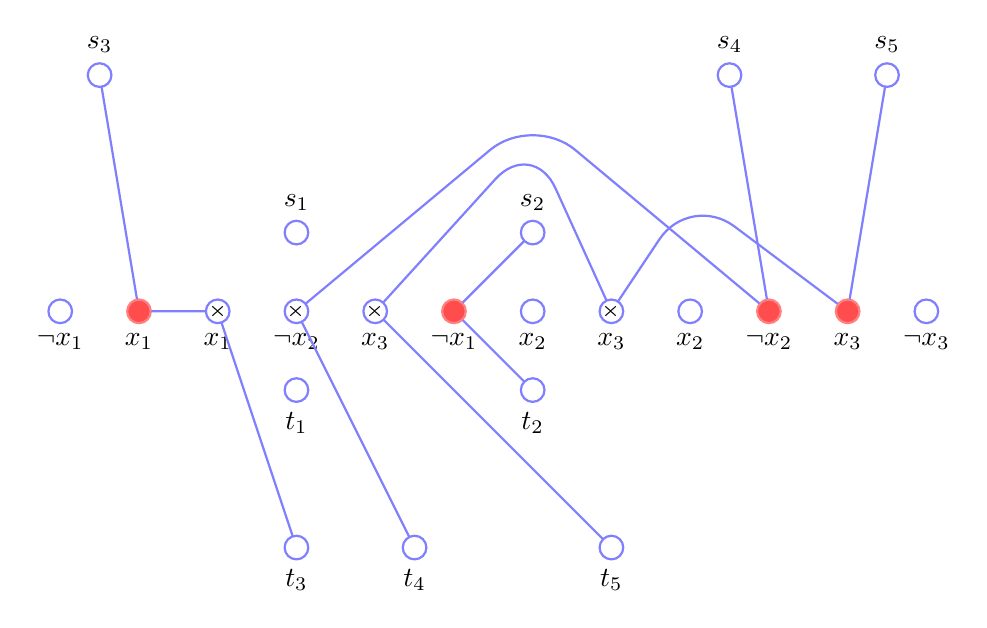
\begin{tikzpicture}
    [mine/.style={circle, draw=red!50,fill=red!70,thick,inner sep=0pt,minimum size=6mm,scale=0.5},
    empty/.style={circle, draw=blue!50,thick,inner sep=0pt,minimum size=6mm,scale=0.5}]
    \node[empty,label=below:{$x_1$}] (x11) at (0,0) {\Large\textbf{{×}}};
    \node[empty,label=below:{$\lnot x_2$}] (x12) at (1,0) {\Large\textbf{{×}}};
    \node[empty,label=below:{$x_3$}] (x13) at (2,0) {\Large\textbf{{×}}};
    \node[empty,label=above:{$s_1$}] (s1) at (1,1) {};
    \node[empty,label=below:{$t_1$}] (t1) at (1,-1) {};

    \node[mine,label=below:{$\lnot x_1$}] (x21) at (3,0) {};
    \node[empty,label=below:{$x_2$}] (x22) at (4,0) {};
    \node[empty,label=below:{$x_3$}] (x23) at (5,0) {\Large\textbf{{×}}};
    \node[empty,label=above:{$s_2$}] (s2) at (4,1) {};
    \node[empty,label=below:{$t_2$}] (t2) at (4,-1) {};

    \node[mine,label=below:{$x_1$}] (x31) at (-1,0) {};
    \node[empty,label=below:{$\lnot x_1$}] (nx31) at (-2,0) {};
    \node[empty,label=above:{$s_3$}] (s3) at (-1.5,3) {};
    \node[empty,label=below:{$t_3$}] (t3) at (1,-3) {};

    \node[empty,label=below:{$x_2$}] (x42) at (6,0) {};
    \node[mine,label=below:{$\lnot x_2$}] (nx42) at (7,0) {};
    \node[empty,label=above:{$s_4$}] (s4) at (6.5,3) {};
    \node[empty,label=below:{$t_4$}] (t4) at (2.5,-3) {};

    \node[mine,label=below:{$x_3$}] (x53) at (8,0) {};
    \node[empty,label=below:{$\lnot x_3$}] (nx53) at (9,0) {};
    \node[empty,label=above:{$s_5$}] (s5) at (8.5,3) {};
    \node[empty,label=below:{$t_5$}] (t5) at (5,-3) {};

    %\draw [blue!50,thick] (s1) -- (x11);
    %\draw [blue!50,thick] (s1) -- (x12);
    %\draw [blue!50,thick] (s1) -- (x13);
    %\draw [blue!50,thick] (t1) -- (x11);
    %\draw [blue!50,thick] (t1) -- (x12);
    %\draw [blue!50,thick] (t1) -- (x13);

    \draw [blue!50,thick] (s2) -- (x21);
    %\draw [blue!50,thick] (s2) -- (x22);
    %\draw [blue!50,thick] (s2) -- (x23);
    \draw [blue!50,thick] (t2) -- (x21);
    %\draw [blue!50,thick] (t2) -- (x22);
    %\draw [blue!50,thick] (t2) -- (x23);

    \draw [blue!50,thick] (s3) -- (x31);
    %\draw [blue!50,thick] (s3) -- (nx31);

    %\draw [blue!50,thick] (s4) -- (x42);
    \draw [blue!50,thick] (s4) -- (nx42);

    \draw [blue!50,thick] (s5) -- (x53);
    %\draw [blue!50,thick] (s5) -- (nx53);
    %\draw [blue!50,thick] (t5) -- (nx53);

    \draw [blue!50,thick,rounded corners=20pt] (x31) -- (x11) -- (t3);
    %\draw [blue!50,thick,rounded corners=20pt] (nx31) -- (1,2)-- (x21) -- (t3);

    %\draw [blue!50,thick,rounded corners=20pt] (x42) -- (5,0.5) -- (x22) -- (t4);
    \draw [blue!50,thick,rounded corners=20pt] (nx42) -- (4,2.5) -- (x12) -- (t4);

    \draw [blue!50,thick,rounded corners=20pt] (x53) -- (6,1.5) -- (x23) -- (4,2.2) -- (x13) -- (t5);

\end{tikzpicture}
\caption{When $\{x_1=false,x_2=true,x_3=false\}$, $s_1$ can't reach $t_1$, failed.}
\end{figure}

Similarly, if we already have $k$ node-disjoint paths in graph $G$, we just do the inverse process, the $3SAT$ can be satisfied.

Directed Disjoint Paths Problem is in \textbf{NP}-complete.

\section*{6\quad Longest Common Subsequence Problem}

First, Longest Common Subsequence is in \textbf{NP}. Given an integer $k$ and a set $R=\{S_1,S_2,...,S_p\}$ of sequences, whose $length(S_i)=n$. We can verify if $|LCS(R)|\geq k$ in polynomial time. Just check whether each subsequence $s$ of $S_1$ is also the subsequence of $S_2,...,S_p$, it takes $O(C_n^k*n*(p-1))$.

Second, we prove $Vertex~Cover \leq_p LCS$. Given $G=<E,V>$ where $V=\{1,2,...,n\}$ and $E=e_{ij}$, $i,j\in V$. For each edge $e_{ij}$, we construct a sequence $S_{ij}=1,2,...,i-1,i+1,...n,1,2,...,j-1,j+1,...n$, $R=\{S_{ij}|e_{ij}\in E\}$. If there are $k$ vertexes can cover all $e_{ij}$, then $|LCS(R)|\geq n-k$ holds. What's more, $V-T$ can be the $LCS(R)$ where $T$ is the vertexes that can cover all edges in $G$.

Given a graph $G$ like Figure 8, we can list all the $S_{ij}$ on the right side.

\begin{figure}[!ht]
\centering
\parbox{1in}
{
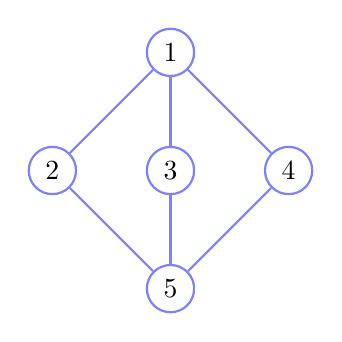
\begin{tikzpicture}
    [mine/.style={circle, draw=red!50,fill=red!70,thick,inner sep=0pt,minimum size=6mm},
    empty/.style={circle, draw=blue!50,thick,inner sep=0pt,minimum size=6mm}]
    \node[empty] (v3) at (0,0) {3};
    \node[empty] (v2) at (-1.5,0) {2};
    \node[empty] (v4) at (1.5,0) {4};
    \node[empty] (v1) at (0,1.5) {1};
    \node[empty] (v5) at (0,-1.5) {5};

    \draw [blue!50,thick] (v1) -- (v2);
    \draw [blue!50,thick] (v1) -- (v3);
    \draw [blue!50,thick] (v1) -- (v4);
    \draw [blue!50,thick] (v5) -- (v2);
    \draw [blue!50,thick] (v5) -- (v3);
    \draw [blue!50,thick] (v5) -- (v4);
\end{tikzpicture}
}
\qquad
\begin{minipage}{3in}
\[
=>~~
\begin{array}{ccl}
V&=&1,2,3,4,5\\
S_{12}&=&2,3,4,5,1,3,4,5\\
S_{13}&=&2,3,4,5,1,2,4,5\\
S_{14}&=&2,3,4,5,1,2,3,5\\
S_{25}&=&1,3,4,5,1,2,3,4\\
S_{35}&=&1,2,4,5,1,2,3,4\\
S_{45}&=&1,2,3,5,1,2,3,4
\end{array} \nonumber
\]
\end{minipage}
\caption{Graph $G$ for vertex cover.}
\end{figure}

There are three vertexes that can cover all the edges, i.e. $k=3$ and $T=\{2,3,4\}$, so $|LCS(R)|\geq n-k=2$ holds. What's more, $LCS=\{1,5\}$.

If vertexes cover is $T=\{2,3,4\}$, we prove $LCS=\{1,5\}$. As vertexes cover is $T=\{2,3,4\}$, for $\forall e_{ij}$, either $i\in T$ or $j\in T$. If $i\in T$, set $S_{ij}=1,2,...,i-1,i+1,...n$; else if $j\in T$, set $S_{ij}=1,2,...,j-1,j+1,...n$. So $LCS(R)=V-T$. For example, for $e_{12}$, $2\in T$, we set $S_{12}=1,3,4,5$, so $2\notin LCS$. Finally $LCS=\{1,5\}$.

If $LCS=\{1,5\}$, we prove $T=\{2,3,4\}$ is vertexes cover. If there is one edge that $T$ can't cover, say $e_{ij}$. so $i\notin T$ and $j\notin T$. $S_{ij}=1,2,...,i-1,i+1,...n,1,2,...,j-1,j+1,...n$, $LCS(S_{ij},V)\nsupseteqq LCS(R)$, contradiction! For example, suppose edge $e_{15}$ exists, $e_{15}$ can't be covered by $T$, $S_{15}=2,3,4,5,1,2,3,4$, $V=1,2,3,4,5$. $LCS(S_{15},V)\nsupseteqq LCS(R)=\{1,5\}$, so $e_{15}$ doesn't exist, $T$ is vertexes cover.

%http://tex.stackexchange.com/questions/8652/what-does-t-and-ht-mean
\begin{figure}[!ht]
\centering
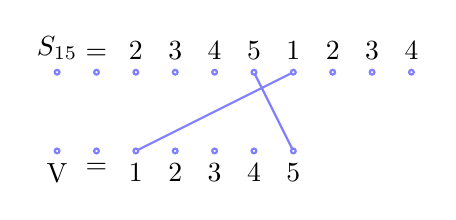
\begin{tikzpicture}
    [empty/.style={circle, draw=blue!50,thick,inner sep=0pt,minimum size=6mm,scale=0.1}]
    \node[empty,label=above:{$S_{15}$}] (s) at (0,0) {};
    \node[empty,label=above:{=}] (eq1) at (0.5,0) {};
    \node[empty,label=above:{2}] (v2) at (1,0) {};
    \node[empty,label=above:{3}] (v3) at (1.5,0) {};
    \node[empty,label=above:{4}] (v4) at (2,0) {};
    \node[empty,label=above:{5}] (v5) at (2.5,0) {};
    \node[empty,label=above:{1}] (v11) at (3,0) {};
    \node[empty,label=above:{2}] (v22) at (3.5,0) {};
    \node[empty,label=above:{3}] (v33) at (4,0) {};
    \node[empty,label=above:{4}] (v44) at (4.5,0) {};

    \node[empty,label=below:{V}] (v) at (0,-1) {};
    \node[empty,label=below:{=}] (eq2) at (0.5,-1) {};
    \node[empty,label=below:{1}] (v111) at (1,-1) {};
    \node[empty,label=below:{2}] (v222) at (1.5,-1) {};
    \node[empty,label=below:{3}] (v333) at (2,-1) {};
    \node[empty,label=below:{4}] (v444) at (2.5,-1) {};
    \node[empty,label=below:{5}] (v555) at (3,-1) {};

    \draw [blue!50,thick] (v11) -- (v111);
    \draw [blue!50,thick] (v5) -- (v555);

\end{tikzpicture}
\caption{There is one intersection, so $LCS(S_{15},V)\nsupseteqq LCS(R)=\{1,5\}$, $e_{15}$ doesn't exist, $T=\{2,3,4\}$ is vertexes cover.}
\end{figure}

So, the $yes/no$ \textbf{LCS} problem is in \textbf{NP}-complete.
\end{document}
